
\chapter{Introducción}
\label{cha:introduccion}

\begin{FraseCelebre}
  \begin{Frase}
    La mayoría de las personas gastan más tiempo y energías en hablar de los problemas que en afrontarlos.
  \end{Frase}
  \begin{Fuente}
    Henry Ford
  \end{Fuente}
\end{FraseCelebre}

\section{Motivación}
\label{sec:motivacion}

El desarrollo de sistemas de videovigilancia automatizados ha despertado un gran interés en los últimos años en la monitorización de lugares públicos y privados. Conforme que estos sistemas crecen, la forma de observar todas las cámaras en un momento concreto se convierte en todo un desafío, especialmente en lugares públicos y concurridos como pueden ser aeropuertos, estaciones de trenes o edificios. Una característica muy deseable de estos sistemas es la detección automática de eventos de interés, característica la cual permite centrar la atención en ubicaciones de vigilancia potencialmente peligrosas.

En los últimos años la \gls{doa} se ha investigado para detectar eventos de gran interés como objetos abandonados \cite{filonenko2016unattended} y vehículos estacionados ilegalmente \cite{Wahyono2017CumulativeDF}. Los sistemas \gls{doa} analizan los objetos que se encuentran en movimiento en un determinado escenario con el objetivo de identificar los estáticos, los cuales se convierten en los aspirantes a ser objetos abandonados. Posteriormente, una serie de pasos de filtrado validan a los candidatos para determinar si son vehículos, personas u objetos abandonados.

Los desarrollos de técnicas de \gls{doa} se encuentran constantemente enfrentados contra diferentes desafíos durante su implementación. Es necesario que funcionen correctamente en escenarios complejos con condiciones cambiantes y una alta densidad de objetos en movimiento. Muchos factores visuales afectan el rendimiento de \gls{doa}, como el ruido de la imagen, cambios en la iluminación, ya sean graduales o inesperados, fluctuación de la cámara y camuflaje entre un primer plano del objeto y el fondo son algunos de los desafíos de \textit{background substraction}. Fondos dinámicos, que contienen objetos en movimiento, también son un tema importante a tener en cuenta. Además, los desafíos con el procesamiento de datos en tiempo real surgen por la gran cantidad de datos que deben de ser manejados por los (relativamente) complejos sistemas \gls{doa} compuestos por varias etapas. Otro desafío crítico es la operación sin supervisión durante largos períodos de tiempo donde el efecto de los factores visuales disminuyen el rendimiento y los errores suelen aparecer en las primeras etapas de los sistemas de \gls{doa}, que se propagan a las etapas posteriores.

Los sistemas de \gls{doa} actuales se centran principalmente en dos etapas principales: detección estacionaria y clasificación de objetos. La tarea de detección de objetos estáticos tiene como objetivo detectar en el primer plano los objetos de la escena que permanecen inmóviles después de haberse movido anteriormente. Una vez ubicados los objetos estacionarios, la tarea de clasificación identifica si el objeto estático se trata de un objeto abandonado o no. A pesar de la gran variedad de propuestas, hay una falta de comparaciones cruzadas (tanto teóricas como experimentales), lo que dificulta la evaluación. Además, estos enfoques proporcionan soluciones parciales para los sistemas de \gls{doa}, ya que solo se estudia una etapa de la tubería completa. El impacto de estas soluciones parciales rara vez se estudia para sistemas \textit{end-to-end} más grandes, cuya entrada es la secuencia de vídeo y la salida es el evento del objeto abandonado. Las validaciones experimentales generalmente se limitan a vídeos de corta duración o de baja complejidad. Por lo tanto, los parámetros del sistema pueden estar ajustados en exceso a los desafíos específicos que aparecen en los datasets pequeños, lo cual dificulta la extrapolación de conclusiones a datos no vistos.

Los objetos abandonados se pueden determinar mediante dos reglas: el objeto aspirante se encuentra estático o desatendido. El primer enfoque corresponde a una regla espacial, en la que un objeto se considera desatendido si el propietario del objeto se encuentra apartado del objeto. La cercanía al objeto se define considerando una elipse o círculo cuyo radio es proporcional al tamaño del objeto. En \cite{Lv06leftluggage} se establece una distancia máxima de 3 metros para evaluar si el objeto es abandonado o no al pasar 30 segundos, tal como se muestra en la figura \ref{fig:pets2006-3m}.

\begin{figure}[ht]
\centering
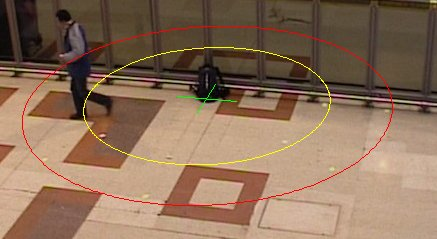
\includegraphics[width=0.45\textwidth]{img/chapters/introduccion/pets2006-3m.jpeg}
\caption{\label{fig:pets2006-3m}Persona cruzando del radio de 2 metros (marcado en amarillo) al radio de 3 metros (marcado en rojo) alrededor de su equipaje (marcado con una cruz verde) \cite{7789647}}
\end{figure}

El segundo enfoque define una regla temporal en la que un objeto se considera estacionario si se encuentra inmóvil durante un cierto período de tiempo, dependiendo de la aplicación, siendo típicamente 30 o 60 segundos. Ambas reglas se deben de cumplir para considerar un evento de objeto abandonado. Los sistemas \gls{doa} propuestos en la literatura se pueden unificar utilizando el diagrama de la figura \ref{fig:canonical-framework-aod}

\begin{figure}[ht]
\centering
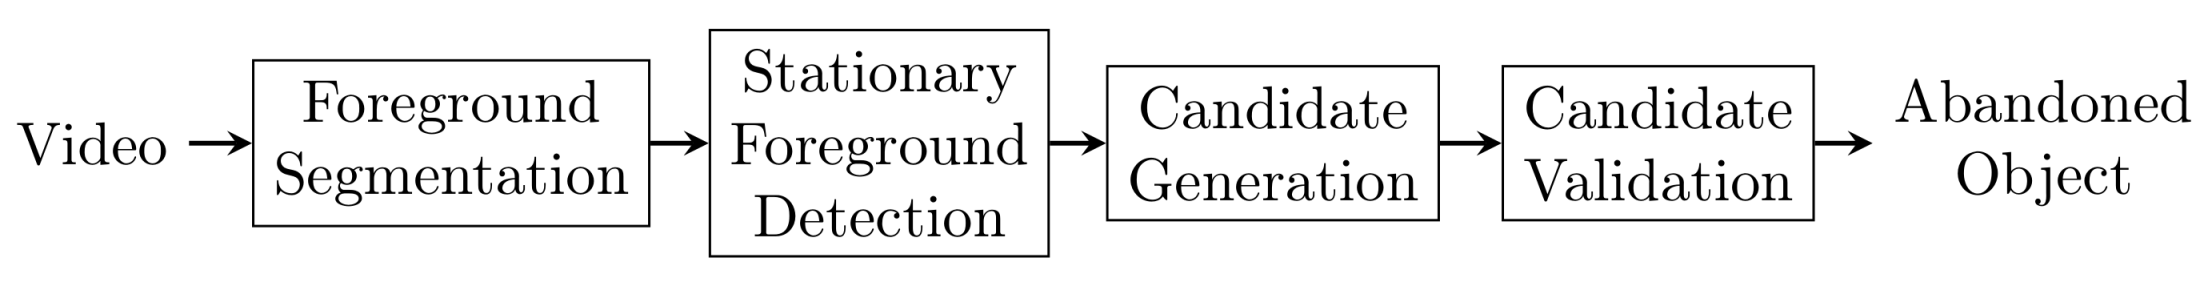
\includegraphics[width=0.75\textwidth]{img/chapters/introduccion/canonical-framework-aod.png}
\caption{\label{fig:canonical-framework-aod}Marco de referencia en detección de objetos abandonados}
\end{figure}

Este diagrama está formado por varias etapas para la segmentación del primer plano (es decir, detectar las \gls{roi}), detección de primer plano estacionaria (es decir, determinar cuáles no se mueven durante un cierto período de tiempo), la generación de posibles candidatos (es decir, la identificación de los objetos aspirantes a ser abandonados), y validación del candidato (es decir, decidir si el objeto ha sido abandonado o no). Las primeras dos etapas pueden ser aplicables mediante la regla temporal antes mencionada y la tercera y cuarta etapa con la regla espacial. El rendimiento de cada etapa está directamente relacionada con la de la etapa anterior por lo que, las investigaciones de \gls{doa} están enfocadas hacia la primera y segunda etapa.

En los últimos años se ha mostrado un gran progreso en la detección de personas debido a la aparición de métodos de aprendizaje profundo \cite{benenson2014years} \cite{zhang2016far} \cite{hosang2015taking}. Los detectores de personas y objetos basados en las \gls{cnn} pueden aprender características de píxeles sin procesar, superando modelos basados en características hechas a mano. Los enfoques de dos etapas primero calculan los métodos de propuesta de región sobre la entrada para calcular los potenciales cuadros delimitadores que se clasifican en segundo lugar. Los enfoques de \gls{r-cnn} \cite{girshick2014rich} \cite{ren2016faster} son actualmente uno de los métodos de dos etapas de detección superiores. Por otro lado, los enfoques de una sola etapa replantean las dos etapas (propuesta de región y clasificación) en un problema de regresión de una sola etapa, lo que requiere menos tiempo. Cuatro modelos de etapa única de última generación son SqueezeDet \cite{wu2019squeezedet}, \gls{yolo} \cite{redmon2016look}, \gls{ssd} \cite{Liu_2016} y \gls{dssd} \cite{fu2017dssd}.

Algunos sistemas de detección de objetos abandonados del Estado del Arte no incluyen la etapa de detección de personas, ya que no consideran detecciones falsas causadas por personas inmóviles. Alternativamente, otros trabajos incorporan una etapa de detección de personas para la clasificación de candidatos. El clasificador de cuerpo completo de características similares a Haar, descrito en \cite{990517}, es un clasificador basado en un modelo de persona; por tanto, es muy eficaz. Se utiliza en el sistema de detección de objetos abandonados propuesto en \cite{LIN2016181}. El modelo deformable basado en partes, propuesto en \cite{5255236}, es un modelo de persona basado en partes, que fue utilizado en \cite{7052354} para la detección de personas. Dependiendo del propósito, los candidatos pueden restringirse a una categoría de objeto, como coches; por lo tanto, se requiere un detector/clasificador específico. El \gls{hog} aplica una búsqueda exhaustiva basada en descriptores de apariencia a lo largo de toda la imagen. Se utilizó para la detección de automóviles en \cite{Wahyono2017CumulativeDF}, aunque inicialmente se propuso en \cite{1467360} para la detección humana. Todas las tecnologías mencionadas anteriormente estaban basadas en la apariencia, pero esto también se puede combinar con seguimiento para la detección de personas, como se hizo en \cite{5571035}. La figura \ref{fig:diagram-stationary-detection} muestra un diagrama de bloques de esta etapa, donde se ilustra el funcionamiento.

\begin{figure}[ht]
\centering
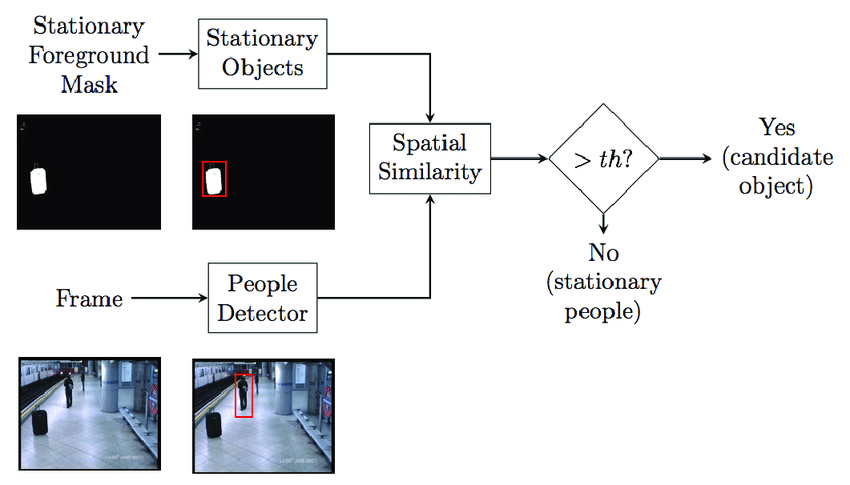
\includegraphics[width=0.65\textwidth]{img/chapters/introduccion/Block-diagram-Stationary-detection.png}
\caption{\label{fig:diagram-stationary-detection}Diagrama de bloques del módulo de generación de candidatos}
\end{figure}

\section{Objetivos}
\label{sec:objetivos}

El objetivo que se persigue es el desarrollo de una estrategia de detección de objetos abandonados mediante el uso de \cite{confusion-matrix} en aplicaciones de videovigilancia. En concreto se va a estudiar cuando se ha abandonado los siguientes tipos de objetos: mochilas, bolsos, maletines, bolsas de mano y maletas. Los espacios donde se va a evaluar la eficacia del sistema de detección desarrollado será tanto interiores como exteriores: aeropuertos, estaciones de metro, interiores y exteriores de edificios o cualquier tipo de infraestructura que disponga de una o varias cámaras de videovigilancia.

Los pasos para abordar este problema son los siguientes.

\begin{itemize}
    \item \textbf{Revisión del Estado de Arte}. Búsqueda y estudio de estrategias en la identificación de objetos abandonados en aplicaciones de videovigilancia dentro del Estado del Arte actual para tener un punto de partida. Por otro lado se deberá de buscar los datasets más relevantes en la evaluación de detección de objetos abandonados.
    \item \textbf{Evaluación de algoritmos de detección de objetos más relevantes}. Se estudiará y comparará los algoritmos de detección de objetos actuales y se argumentará el motivo de la elección de uno concreto. Una vez seleccionado el algoritmo de detección se deberá de evaluar si trabajar sobre un dataset conocido o si por el contrario es interesante el entrenamiento de una red neuronal personalizada en la que se detecten solamente los objetos de interés. La elección del dataset de referencia para la evaluación del algoritmo de detección se decidirá teniendo en cuenta las principales métricas de clasificación de \textit{Machine Learning}. Teniendo un dataset de referencia seleccionado, se ejecutará el algoritmo sobre los datasets más utilizados en evaluación de algoritmos de detección de objetos abandonados.
    \item \textbf{Evaluación de algoritmos de seguimiento o \textit{tracking} de objetos más relevantes}. En base al modelo del algoritmo de detección de objetos seleccionado se estudiará y evaluará los algoritmos de seguimiento actuales. El objetivo de este punto es que en la detección de objetos y personas, cada elemento tenga una identidad propia a lo largo del tiempo, o lo que es lo mismo, a lo largo de los fotogramas de un vídeo. De tal manera que, cuando se implemente el algoritmo de detección de objetos abandonados sea más sencillo la asociación de persona-objeto. De igual manera que en el algoritmo de detección, también se ejecutará el algoritmo en los datasets más relevantes en detección de objetos abandonados para evaluar el rastreo sobre personas y objetos de interés a lo largo de un vídeo.
    \item \textbf{Implementación y evaluación de un algoritmo de detección de objetos abandonados}. Se desarrollará un algoritmo capaz de determinar si un objeto ha sido abandonado o no. Existen tres posibles escenarios. El primero es que el objeto se encuentre móvil durante toda la ejecución del vídeo y no se pueda asociar a ninguna persona como propietario. La segunda es que a una persona a la que se le ha asociado un objeto se alejen más de una cierta distancia a lo largo de un número determinado de fotogramas. La tercera es que a una persona a la que se le ha asociado un objeto desaparezca y se esté detectando únicamente el objeto durante un número determinado de fotogramas. Para estos dos últimos casos se deberá de establecer una asociación persona-objeto y estudiar su comportamiento a lo largo del vídeo.
\end{itemize}

\section{Estructura de la memoria}
\label{sec:estructura-memoria}
En este apartado se resume brevemente como se encuentra organizados los contenidos que componen el presente \gls{tfm}.

\begin{itemize}
    \item \textbf{Capítulo \ref{cha:introduccion}: Introducción.} Se expondrá la motivación que ha impulsado la realización de este \gls{tfm}. Se citará brevemente trabajos previos que han servido de esqueleto del proyecto. Por otro lado se argumentarán los objetivos que se pretenden alcanzar.
    \item \textbf{Capítulo \ref{cha:estudio-teórico}: Estudio teórico.} Se realizará un estudio exhaustivo del Estado del Arte en lo referente a los métodos de detección de objetos abandonados que se han empleado en los últimos años y se describirán los algoritmos de detección y seguimiento que se utilizarán en el desarrollo del proyecto.
    \item \textbf{Capítulo \ref{cha:desarrollo}: Desarrollo.} Se desarrollará la implementación de los algoritmos que se van a utilizar para la detección y rastreo de personas y objetos así como el algoritmo de detección de objetos abandonados.
    \item \textbf{Capítulo \ref{cha:resultados}: Resultados.} Se expondrán los resultados obtenidos en base a métricas de calidad y los datasets utilizados para la evaluación de los algoritmos.
    \item \textbf{Capítulo \ref{cha:concl-lineas-futuras}: Conclusiones y líneas futuras.} Se detallarán las conclusiones que se han llegado al finalizar este proyecto. Se explicarán las ventajas y limitaciones que presenta la idea propuesta para su desarrollo. Por otro lado se razonarán posibles vías de desarrollo derivadas de este proyecto, así como nuevos proyectos donde se puedan emplear el mismo algoritmo de detección y seguimiento y solamente se tenga que programar un algoritmo que realice una función concreta.
    \item \textbf{Bibliografía.} Se incluirán cada uno de los artículos, repositorios, datasets y toda clase de material consultado para la elaboración de este \gls{tfm}. 
    \item \textbf{Apéndice \ref{cha:pliego-de-condiciones}.} Se hará referencia al pliego de condiciones donde se tendrán en cuenta las especificaciones \textit{hardware} y \textit{software} que se han empleado en el desarrollo de este proyecto.
    \item \textbf{Apéndice \ref{cha:presupuesto}.} Se mostrará el presupuesto donde se incluye los costes materiales \textit{hardware} y \textit{software} y el coste de la mano de obra en función a la duración estimada del proyecto.
    \item \textbf{Apéndice \ref{cha:manual-usuario}.} Este apéndice se dividirá en dos partes. Primero, en guía de instalación, se detallarán cada uno de los pasos en la instalación de las dependencias necesarias para el correcto funcionamiento de los algoritmos. Posteriormente, se podrá consultar la guía de ejecución, donde se indicará como poner en funcionamiento cada uno de los algoritmos desarrollados en este proyecto.
\end{itemize}




